\documentclass{article}

\textwidth=6.5in
\textheight=8.5in
\voffset=-54pt
\oddsidemargin=0in
\evensidemargin=0in
\setlength{\parskip}{8pt}
\setlength{\parindent}{0pt}

\usepackage{amsmath, amssymb}
\usepackage{ifthen}

\usepackage[inline]{enumitem}
\setlist{topsep=0pt, parsep=8pt}

\usepackage[rgb,table]{xcolor}\convertcolorsUfalse
\usepackage{graphicx}

% change hyperref options
\PassOptionsToPackage{hyphens}{url}
\usepackage[bookmarks,colorlinks,linkcolor=black,citecolor=blue,pdfstartview=FitH,urlcolor=blue]{hyperref}
\hypersetup{pdfpagemode=UseNone}
\usepackage{bookmark}

\usepackage{graphicx}
\usepackage{multicol}
\usepackage{framed}
\usepackage{array}

\usepackage{icomma}

\usepackage{soul}
\usepackage[normalem]{ulem}

\usepackage{pgfplots}
\pgfplotsset{compat=1.18}  
\pgfplotscreateplotcyclelist{mycolor}{black, blue, red, green!70!black, magenta, purple, cyan, orange }  
\pgfplotsset{
  disabledatascaling,
  cycle list=tikzcolor, 
  axis lines=middle,
  every axis plot/.style={no marks, thick},
  every axis/.style={
    enlarge x limits=false,
    enlarge y limits=auto,
    xlabel style={at={(current axis.right of origin)},anchor=west},
    ylabel style={at={(current axis.above origin)},anchor=south},
    % extra x and y ticks for asymptotes
    extra x tick style={grid=major, grid style={dashed,black}},
    extra y tick style={grid=major, grid style={dashed,black}},
    /pgf/number format/1000 sep={},
  },    
  tick label style = {font=\footnotesize, fill=\currentbgcolor, inner sep=0pt},    
  xticklabel shift=1pt,    
  scaled ticks=false,
  scaled y ticks=false,
  unbounded coords=jump,
  samples=101,
  minor tick length=0,
  scatter/classes={
    open={mark=*,draw=black,fill=white, mark size=2, thin},
    closed={mark=*,draw=black,fill=black, mark size=2, thin}
  },
  width=3in,
}
\pgfplotsset{open/.style={only marks, mark=*, fill=white, thin, mark size=2}}
\pgfplotsset{closed/.style={only marks, mark=*, draw=black, fill=black,
    thin, mark size=2}}
\pgfplotsset{labeled/.style={nodes near coords, only marks, mark=*, draw=black, fill=black, thin, mark size=2, point meta=explicit symbolic}}

\newcommand{\axes}[1][]{
  \begin{tikzpicture}
    \begin{axis}[xtick=\empty, ytick=\empty, ymin=-2, ymax=2,
      xmin=-4.25, xmax=4.25, #1]
    \end{axis}
  \end{tikzpicture}
}
\usepackage{tikz}
\usetikzlibrary{
  matrix,%
  % enables the snake paths
  decorations.pathmorphing,%
  % enables bigger arrows
  decorations.markings,%
  decorations.pathreplacing,%
  decorations.text,%
  calc,%
  patterns,%
  shapes.geometric,%
  arrows,
  decorations.shapes,
  positioning,
  plotmarks,
  intersections
}
\tikzset{>=latex} % sets default arrow type in tikz
\tikzset{font=\normalsize}
\tikzset{mark size=1.5pt, mark options=thin}
\tikzset{pin distance=4pt,
  every pin edge/.style={<-, thin, shorten <= -2pt}}

\interfootnotelinepenalty=10000
\renewcommand{\thefootnote}{(\arabic{footnote})}

\newcommand*\colorcircled[2]{\tikz[baseline=(char.base)]{
    \node[shape=circle,draw,inner sep=2pt, #1] (char) {\color{black}#2};}
}

\usepackage{multirow, bigdelim}

% change to \usepackage[sols]{handout} to see solutions
\usepackage[]{handout}

\newcommand\iscurrentenumi[1]{%
  \ifthenelse{\equal{#1}{\theenumi}}{}{#1}}
\setenumerate[1]{ref=\#\arabic*}
\setenumerate[2]{ref=\protect\iscurrentenumi{\theenumi}(\alph*)}
\newcommand\enumiiprefix[2]{%
  \ifthenelse{{\equal{#1}{\theenumi}}\AND{\equal{#2}{(\alph{enumii})}}}{}{}%
  \ifthenelse{{\equal{#1}{\theenumi}}\AND{\NOT{\equal{#2}{(\alph{enumii})}}}}{#2}{}%
  \ifthenelse{\equal{#1}{\theenumi}}{}{#1#2}%
}
\setenumerate[3]{ref=\protect\enumiiprefix{\theenumi}{(\alph{enumii})}\roman*}

\newlength{\tipmargin}
\makeatletter

\newdimen\SOUL@dimen %new
\def\SOUL@ulunderline#1{{%
    \setbox\z@\hbox{#1}%
    % \dimen@=\wd\z@
    \SOUL@dimen=\wd\z@ %new
    \dimen@i=\SOUL@uloverlap
    \advance\SOUL@dimen2\dimen@i %\dimen@ exchanged too
    \rlap{%
      \null
      \kern-\dimen@i
      % \SOUL@ulcolor{\SOUL@ulleaders\hskip\dimen@}%
      \SOUL@ulcolor{\SOUL@ulleaders\hskip\SOUL@dimen}% new
    }%
    \unhcopy\z@
  }}

\renewenvironment{framed}{
  \setlength{\tipmargin}{\textwidth-\linewidth}
  \advance\@totalleftmargin-\tipmargin
  \def\FrameCommand{\hspace{\tipmargin}\fbox}%
  \advance\linewidth\tipmargin
  \MakeFramed {\advance\hsize-\width \FrameRestore}%
}
{\endMakeFramed}

\makeatother

\definecolor{purple}{rgb}{0.5,0,1.0}

\definecolor{skyblue}{rgb}{0, 0.5, 1}

\usepackage{fourier-orns}
\newcommand{\warningsign}{\tikz[baseline=-4pt]\draw (0, 0) node{\warning};\ignorespaces}

\usepackage{fancyhdr}
\lhead{\textcolor{white}{This content is protected and may not be shared, uploaded, or distributed.}}
\rhead{}
\rfoot{\vspace*{\fill}\footnotesize\textcopyright{} \emph{Harvard Math Ma}}
\renewcommand{\headrulewidth}{0pt}
\pagestyle{fancy}
\begin{document}

\htitle{36. Comparing Exponentials, Logarithms, and Power Functions}

\begin{problemonly}
  \begin{framed}

You should be able to:
    \begin{itemize}[topsep=0pt,partopsep=0pt,parsep=8pt,itemsep=0pt]
    \item Describe the relative growth rates of logarithmic functions, power functions (functions of the form $f(x) = x^p$ where $p$ is a constant), and exponential functions, and use these to calculate limits.    

    \end{itemize}
  \end{framed}
\end{problemonly}

\begin{enumerate}
\item  \emph{Warm up.}

\begin{framed}
{\bf Recall from earlier in the term:} When reasoning about limits to infinity, we want to make use of two big ideas:\begin{itemize} 
\item  that one term ``eventually grows much faster than" another, which is represented by the symbol ``$>>$"
\item that one function ``behaves like" another function, which is represented by the symbol ``$\sim$".
\end{itemize}
Complete reasoning, (which you'll be asked to show in the future) requires: (1) identifying the fastest growing term in different parts of the function, (2) identifying which simplified function the given function behaves like, (3) computing the simplified function's limit, which computes our original function's limit.
\end{framed}

  \begin{enumerate}
  \item

    \note{I want to emphasize a few things:
      \begin{itemize}
      \item Why it's reasonable to just keep the fastest-growing terms. (I will go back to a concrete example like $10^{200} + 10^{50} \approx 10^{200}$.)
      \item Why we know $\displaystyle \lim_{x \to \infty} \dfrac{2x^5}{3x^6} = 0$. At this point, I think a lot of students just have the idea that this is because the numerator has a smaller degree than the denominator, so I want to remind them that the justification really comes from algebraic simplification: $\displaystyle \lim_{x \to \infty} \dfrac{2x^5}{3x^6} = \lim_{x \to \infty} \dfrac{2}{x} = 0$.
      \item Proper notation: it isn't meaningful to write $\dfrac{2 \infty^5}{3 \infty^6}$. I will encourage them to write something like this:
        \begin{align*}
          \lim_{x \to \infty} \frac{2x^5 + 7 \sqrt{x}}{3x^6 - x^2} &= \lim_{x \to \infty} \frac{2x^5}{3x^6} \\
          &= \lim_{x \to \infty} \frac{2}{\colorcircled{skyblue}{3x}} \raisebox{-10pt}{\color{skyblue}$\to \infty$} \\
          &= 0
        \end{align*}
      \end{itemize}}

    \begin{problem}[\vfill]
      Evaluate $\displaystyle \lim_{x \to \infty} \frac{2x^5 + 7 \sqrt{x}}{3x^6 - x^2}$, and write a careful justification with correct notation. Why is the method you used valid? 
    \end{problem}

    \begin{solution}
      As $x \to \infty$, the behavior is determined by
      the fastest-growing/dominant terms in the numerator and denominator.
      \begin{align*}
          \lim_{x \to \infty} \frac{2x^5 + 7 \sqrt{x}}{3x^6 - x^2} &= \lim_{x \to \infty} \frac{2x^5}{3x^6} \\
          &= \lim_{x \to \infty} \frac{2}{\colorcircled{skyblue}{$3x$}} \raisebox{-10pt}{\color{skyblue}$\to \infty$} \\
          &= 0
      \end{align*}
    \end{solution}

  \item \label{limit-of-sqrt-over-ln}

    \note{First, I'm just interested to hear whether students have any intuition about this. But mainly, I want to emphasize that all we know at this point is that the numerator and denominator both increase without bound, which isn't enough information to determine the limit.

      I made this problem about $\ln x$ vs.\ $\sqrt{x}$ instead of exponentials vs.\ power functions (which would be the more natural segue into the next problem) because I know some students have the idea that exponential functions grow very quickly; I'm hoping this one will be less familiar to students. 

      Today, we'd like to get a sense of how the main types of functions we've studied relate to each other as $x \to \infty$.
    }

    \begin{problem}[\vfill\newpage]
      What do you think $\displaystyle \lim_{x \to \infty} \dfrac{\sqrt{x}}{\ln x}$ is?
    \end{problem}

    \begin{solution}
      We know that as $x\to\infty$, both $\sqrt{x}$ and $\ln x$ increase
      without bound. Since the numerator and denominator both approach
      $\infty$, we don't know enough right now to determine
      this limit. We need to figure out whether $\sqrt{x}$ or $\ln x$
      grows faster as $x \to \infty$.
    \end{solution}
  \end{enumerate}

\item  

  In this problem, we'll compare the growth of $f(x) = 2^x$ and $g(x) = x^{10}$.
  \begin{enumerate}

  \item

    \note{I have no idea what students will say here, so I'm just interested to hear what their guesses are.}

    \begin{problem}
      Here are graphs of $f(x) = 2^x$ and $g(x) = x^{10}$ on $[0, 50]$. Do you think $f(x) = 2^x$ is the solid graph or the dashed graph? Why? 

      \begin{tikzpicture}
        \begin{axis}[disabledatascaling=false, xtick={50}, ytick=\empty, ymax={2^50}, width=2.25in]
          \addplot+[domain=0:50, dashed] {2^x};
          \addplot+[domain=0:50] {x^10}; 
        \end{axis}
      \end{tikzpicture}
    \end{problem}

    \begin{solution}
      It's not easy to tell by looking at the shape of the
      graph. One way to tell that the graph of $f(x)=2^x$ is the
      dashed graph is that $2^{50}=(2^5)^{10}=32^{10}$, which
      is less than $50^{10}$. 
    \end{solution}

  \item Fill out the following table, expressing each answer as a power of 2 (like $2^7$).
  
    \probonly{
    \begin{tabular}{ c | c | c | c | c | c | c | c | c }
      $x$ & \makebox[0.5in]{2} & \makebox[0.5in]{4} & \makebox[0.5in]{8} & \makebox[0.5in]{16} & \makebox[0.5in]{32} & \makebox[0.5in]{64} & \makebox[0.5in]{128} & \makebox[0.5in]{256} \\
      \hline 
      \tikz \draw (0, 0) node[minimum height=0.4in]{$2^x$}; & & & & & & & \\
      \hline
      \tikz \draw (0, 0) node[minimum height=0.4in]{$x^{10}$}; & & & & & & & 
    \end{tabular}}
    \solonly{
    \begin{tabular}{ c | c | c | c | c | c | c | c | c }
      $x$ & \makebox[0.5in]{2} & \makebox[0.5in]{4} & \makebox[0.5in]{8} & \makebox[0.5in]{16} & \makebox[0.5in]{32} & \makebox[0.5in]{64} & \makebox[0.5in]{128} & \makebox[0.5in]{256} \\
      \hline 
      \tikz \draw (0, 0) node[minimum height=0.4in]{$2^x$}; & $2^2$ &
      $2^4$ & $2^8$ & $2^{16}$ & $2^{32}$ & $2^{64}$ & $2^{128}$ &
      $2^{256}$\\
      \hline
      \tikz \draw (0, 0) node[minimum height=0.4in]{$x^{10}$}; & $2^{10}$
      & $2^{20}$ & $2^{30}$ & $2^{40}$ & $2^{50}$ & $2^{60}$ & $2^{70}$ &
      $2^{80}$
    \end{tabular}}

    \note{We see that $x^{10}$ grows faster than $2^x$ ``at first'', but eventually $2^x$ overtakes $x^{10}$. And we can see that, after this, $2^x$ is going to stay bigger than $x^{10}$ because the pattern in the first row is that the exponent of 2 doubles each time, while the pattern in the second row is that the exponent increases by 10 each time. 

      Here's a GeoGebra applet to illustrate how $2^x$ eventually overtakes $x^{10}$: \url{https://www.geogebra.org/m/je5j6una} Use the slider to zoom.

      I will let students know that we write this as $2^x \gg x^{10}$.}

    \begin{problem}[\vfill]
      Does this change your answer to (a)?
    \end{problem}

    \begin{solution}
      We can see that $2^x$ is initially smaller than $x^{10}$,
      but it eventually grows to be much, much larger than $x^{10}$.
      We write this as $2^x \gg x^{10}$. The graph in part (a)
      ends before showing how $2^x$ overtakes $x^{10}$.
    \end{solution}

  \item

    \begin{problem}[\vfill]
      Based on your table, what do you think $\displaystyle \lim_{x \to \infty} \frac{2^x}{x^{10}}$ is? How about $\displaystyle \lim_{x \to \infty} \frac{x^{10}}{2^x}$?
    \end{problem}

    \begin{solution}
      As $x\to \infty$, since $2^x$ is growing so much faster than
      $x^{10}$, it seems reasonable that 
      $\displaystyle \lim_{x \to \infty} \frac{2^x}{x^{10}} = \infty$
      and
      $\displaystyle \lim_{x \to \infty} \frac{x^{10}}{2^x}=0$.
    \end{solution}

  \end{enumerate}

\end{enumerate}
\note{Now that we've seen a concrete example, we can explain what the $\gg$ notation means in general.}

\begin{problemonly}
  \begin{framed}
    \textbf{Definition.} We say that $g(x)$ \uline{grows faster than} $f(x)$ as $x \to \infty$ if $\displaystyle \lim_{x \to \infty} \frac{g(x)}{f(x)} = \cfitb{0.25in}{\infty}$ or, equivalently, $\displaystyle \lim_{x \to \infty} \frac{f(x)}{g(x)} = \cfitb{0.25in}{0}$. We write this as $g(x) \gg f(x)$.
  \end{framed}
\end{problemonly}

\pspace{\newpage}

\begin{enumerate}[resume]
\item 

  \note{I want students to understand that, since it's possible for a function $f(x)$ to be much smaller than $g(x)$ at first but to eventually overtake it, plugging in a single value of $x$ is never a valid way to evaluate a limit to infinity.}

  \begin{problem}[1in]
    Tyrese would like to evaluate $\displaystyle \lim_{x \to \infty} \dfrac{1.01^x}{x^{1000}}$. He says:
    \begin{quote}
      I used WolframAlpha to plug $x = 1,000,000$ into $\dfrac{1.01^x}{x^{1000}}$; it's about $2 \times 10^{-1679}$, which is really tiny, so the limit is 0. 
    \end{quote}
    Assess Tyrese's reasoning. 
  \end{problem}

    \begin{solution}
      Tyrese's reasoning is not correct. Plugging in $x=10^6$
      to $\dfrac{1.01^x}{x^{1000}}$ gives a small number, but to determine
      the limit as $x\to\infty$, we need to consider what happens
      as $x$ increases \emph{without bound.} If we use WolframAlpha
      to plug in an even
      larger value of $x$, like $x=10^7$, we get around $5 \times 
      10^{36213}$, an extremely large number.
      This indicates that $1.01^x$ eventually grows to be
      much much larger than $x^{1000}$, which we write as
      $1.01^x \gg x^{1000}$, and it means that 
      $\displaystyle \lim_{x \to \infty} \dfrac{1.01^x}{x^{1000}}=\infty$.

      Any exponential growth function $b^x$ (where $b>1$)
      grows faster
      than any power function $x^p$ for $p>0$.
      \end{solution}

  \note{I'll let students know that exponentials with base $>1$ grow faster than $x^p$ for any $p > 0$}


\item 

  \begin{enumerate}
  \item
    \begin{problem}
      Sketch graphs of $f(x) = \log_3 x$ and $g(x) = x^{0.1}$ on the axes below. Label at least three points on each graph with simple coordinates.
    \end{problem}

    \begin{solution}
      \begin{center}
        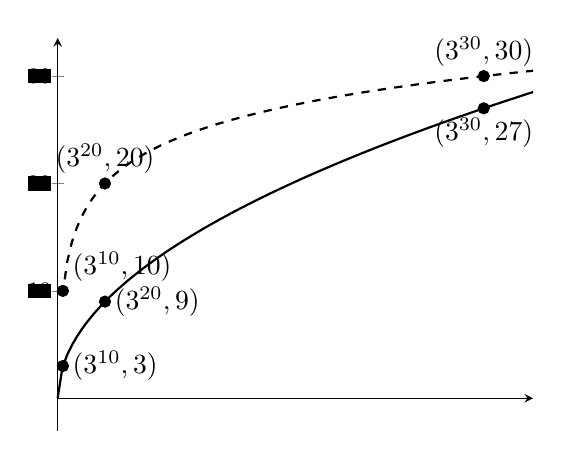
\begin{tikzpicture}
          \begin{axis}[disabledatascaling=false,xtick=\empty, clip=false]
            \addplot[domain=0:3^(6.1), dashed] {ln(x^5)/ln(3)};
            \addplot[domain=0:3^(6.1)] {x^(0.5)};
            \addplot[closed] coordinates {(3^2, 10) (3^4, 20) (3^6, 30) (3^2, 3) (3^4, 9) (3^6, 27)};
            \node[right] at (3^2, 3) {$(3^{10}, 3)$};
            \node[right] at (3^4, 9) {$(3^{20}, 9)$};
            \node[below] at (3^6, 27) {$(3^{30}, 27)$};
            \node[above right] at (3^2, 10) {$(3^{10}, 10)$};
            \node[above] at (3^4, 20) {$(3^{20}, 20)$};
            \node[above] at (3^6, 30) {$(3^{30}, 30)$};
          \end{axis}
        \end{tikzpicture}
      \end{center}
    \end{solution}

    \begin{problemonly}
      \axes[title={$f(x) = \log_3 x$}]
      \hspace{0.25in}
      \axes[title={$g(x) = x^{0.1}$}]
    \end{problemonly}

  \end{enumerate}
  Now, we'll compare the growth rates of $f(x) = \log_{3} x$ and $g(x) = x^{0.1}$.  
  \begin{enumerate}[resume]
  \item Fill out the following table.

    \probonly{
    \begin{center}
      \begin{tabular}{ c *{6}{| c }}
        $x$ & \makebox[0.65in]{$3^{10}$} & \makebox[0.65in]{$3^{20}$} & \makebox[0.65in]{$3^{30}$} & \makebox[0.65in]{$3^{40}$} & \makebox[0.65in]{$3^{50}$} & \makebox[0.65in]{$3^{60}$}  \\
        \hline
        \tikz \draw (0, 0) node[minimum height=0.4in]{$x^{0.1}$}; & & & & & \\
        \hline 
        \tikz \draw (0, 0) node[minimum height=0.4in]{$\log_{3} x$}; & & & & & \\
      \end{tabular}
    \end{center}}
    \pspace{\stretch{0.25}}

    \solonly{
    \begin{center}
      \begin{tabular}{ c *{6}{| c }}
        $x$ & \makebox[0.65in]{$3^{10}$} & \makebox[0.65in]{$3^{20}$} & \makebox[0.65in]{$3^{30}$} & \makebox[0.65in]{$3^{40}$} & \makebox[0.65in]{$3^{50}$} & \makebox[0.65in]{$3^{60}$}  \\
        \hline
        \tikz \draw (0, 0) node[minimum height=0.4in]{$x^{0.1}$}; 
        & $3^1$ & $3^2$ & $3^3$ & $3^4$ & $3^5$ & $3^6$ \\
        \hline 
        \tikz \draw (0, 0) node[minimum height=0.4in]{$\log_{3} x$};
        & $10$ & $20$ & $30$ & $40$ & $50$ & $60$\\
      \end{tabular}
    \end{center}}

  \item
    \begin{problem}[\nstretch{0.25}]
      Based on the table, what's $\displaystyle \lim_{x \to \infty} \frac{\log_{3} x}{x^{0.1}}$? How about $\displaystyle \lim_{x \to \infty} \frac{x^{0.1}}{\log_{3} x}$? 
    \end{problem}

    \begin{solution}
      Based on the table, we can see that eventually, $x^{0.1} \gg
      \log_3 x$, so $\displaystyle \lim_{x \to \infty} \frac{\log_{3} x}{x^{0.1}} = 0$ and $\displaystyle \lim_{x \to \infty} \frac{x^{0.1}}{\log_{3} x} = \infty$.

      Any logarithmic function $\log_b x$ (for $b > 1$) grows more
      slowly than any power function $x^p$ for $p>0$.
    \end{solution}
  \end{enumerate}

  \note{I'll let students know that $\log_b x$ (if $b > 1$) grows more slowly than $x^p$ for any $p > 0$.}
\begin{framed}
\item 

  \begin{problem}
    Fill in the blanks below with the following 3 types of functions:
    \begin{itemize}[nosep]
    \item $x^p$ where $p$ is a positive constant
    \item $b^x$ where $b$ is a constant $> 1$
    \item $\log_b x$ where $b$ is a constant $> 1$
    \end{itemize}
  \end{problem}

  \[ \cfitb{0.75in}{\log_b x} \ll \cfitb{0.75in}{x^p} \ll \cfitb{0.75in}{b^x} \] 
\end{framed}
  \note{The next question is just meant to prompt students to remember that such functions approach 0 as $x \to \infty$.}

  \begin{problem}[0.25in]
    What about $b^x$ with $b < 1$? 
  \end{problem}

  \begin{solution}
    If $b<1$, then $b^x$ is an exponential decay function,
    so as $x\to\infty$, $b^x$ approaches $0$.
  \end{solution}

\item 

  \note{I hope students will have reasonable intuition that, say, $1.1^x \ll 5^x$. If so, we'll just rely on that. If not, we can always check by thinking about $\displaystyle \lim_{x \to \infty} \frac{1.1^x}{5^x}$ or $\displaystyle \lim_{x \to \infty} \frac{5^x}{1.1^x}$.}

  \begin{problem}[\vfill]
    Which of the functions $f(x)$ below have $\displaystyle \lim_{x \to \infty} f(x) = \infty$? Arrange those with $\ll$ signs in between them.
    \[ x^{1000} \hspace{0.3in} \log_5 x \hspace{0.3in} \sqrt[5]{x} \hspace{0.3in} 5^x \hspace{0.3in} x^{-0.1} \hspace{0.3in} 0.9^x \hspace{0.3in} 1.1^x \]
  \end{problem}

  \begin{solution}
    All of the functions except $x^{-0.1}$ and $0.9^x$ increase
    without bound as $x \to \infty$. $\log_5 x$ is a logarithmic function,
    so it grows more slowly than the power functions $\sqrt[5]{x}$ and $x^{1000}$, which grow more slowly than the exponential functions $1.1^x$ and $5^x$. Power functions with higher powers grow faster, so $\sqrt[5]{x}$ grows more slowly than $x^{1000}$. 
    Exponential functions with larger bases grow faster, so
    $1.1^x$ grows more slowly than $5^x$.
    \[\log_5 x \ll \sqrt[5]{x} \ll x^{1000} \ll 1.1^x  \ll 5^x \]
  \end{solution}

  \warningsign These growth rates are only relevant when thinking about what happens as $x \to \infty$!




\item 

  \note{Here, I want to talk about writing justifications: it's fine to write simply ``$\displaystyle \lim_{x \to \infty} \frac{\sqrt{x}}{\ln x} = \infty$ because $\sqrt{x} \gg \ln x$.''}

  \begin{problem}[\vfill]
    With your new knowledge, do \ref{limit-of-sqrt-over-ln}. 
  \end{problem}

  \begin{solution}
    In \ref{limit-of-sqrt-over-ln}, we considered the limit 
    $\displaystyle \lim_{x \to \infty} \frac{\sqrt{x}}{\ln x}$. We now
    know that $\displaystyle \lim_{x \to \infty} \frac{\sqrt{x}}{\ln x} = \infty$, and our justification is that $\sqrt{x} \gg \ln x$. 
  \end{solution}

\begin{framed}
{\bf Remember (yes, again!):} When reasoning about limits to infinity, we want to make use of two big ideas:\begin{itemize} 
\item  that one term ``eventually grows much faster than" another, which is represented by the symbol ``$>>$"
\item that one function ``behaves like" another function, which is represented by the symbol ``$\sim$".
\end{itemize}
Complete reasoning, (which you'll be asked to show in the future) requires: (1) identifying the fastest growing term in different parts of the function, (2) identifying which simplified function the given function behaves like, (3) computing the simplified function's limit, which computes our original function's limit.
\end{framed}
\item Evaluate the following limits. Please write your justifications carefully.

  \begin{enumerate}

  \item

    \note{Again, I want to talk about acceptable justifications. Here, it'd be fine for students to write
      \begin{align*}
        \lim_{x \to \infty} \frac{x^3 + 2x}{e^x + 3x} &= \lim_{x \to \infty} \frac{x^3}{e^x} \\
        &= 0 \text{ since $x^3 \ll e^x$}
      \end{align*}
      }

    \begin{problem}[\vfill\newpage]
      $\displaystyle \lim_{x \to \infty} \frac{x^3 + 2x}{e^x + 3x}$      
    \end{problem}

    \begin{solution}
      As $x\to \infty$, the dominant terms in the numerator and denominator
      are $x^3$ and $e^x$ respectively.
      \begin{align*}
        \lim_{x \to \infty} \frac{x^3 + 2x}{e^x + 3x} &= \lim_{x \to \infty} \frac{x^3}{e^x} \\
        &= 0 \text{ since $x^3 \ll e^x$}
      \end{align*}
    \end{solution}

  \item

    \note{This and the next part are to re-emphasize that the growth rates are only useful when $x \to \infty$.}

    \begin{problem}[\vfill]
      $\displaystyle \lim_{x \to -\infty} \frac{x^3 + 2x}{e^x + 3x}$
    \end{problem}

    \begin{solution}
      As $x\to -\infty$, $e^x$ approaches $0$, so the dominant terms in the numerator and denominator
      are $x^3$ and $3x$ respectively.
      \begin{align*}
        \lim_{x \to -\infty} \frac{x^3 + 2x}{e^x + 3x} &= 
        \lim_{x \to -\infty} \frac{x^3}{3x} \\
        &= \lim_{x \to -\infty} \frac{x^2}{3} \\
        &= \infty
      \end{align*}
    \end{solution}
    

  \item
    \begin{problem}[\vfill]
      $\displaystyle \lim_{x \to 0} \frac{x^3 + 2x}{e^x + 3x}$      
    \end{problem}

    \begin{solution}
      We can plug in $0$ to evaluate the limit.
      \begin{align*}
        \lim_{x \to 0} \frac{x^3 + 2x}{e^x + 3x} &= 
        \frac{0+0}{1 + 0} \\
        &= 0
      \end{align*}
    \end{solution}

  \item

    \begin{problem}[\vfill]
      $\displaystyle \lim_{x \to \infty} \dfrac{x^2 + 5 e^{2x}}{e^{2x} - 1}$
    \end{problem}

    \begin{solution}
      As $x\to \infty$, the dominant terms in the numerator and denominator
      are $5e^{2x}$ and $e^{2x}$ respectively.
      \begin{align*}
        \lim_{x \to \infty} \frac{x^2 + 5 e^{2x}}{e^{2x} - 1} &=
        \lim_{x \to \infty} \frac{5e^{2x}}{e^{2x}} \\
        &= \lim_{x \to \infty} 5 \\
        &= 5
      \end{align*}
    \end{solution}

  \item

    \note{Reminder of handling $\dfrac{\text{non-zero}}{0}$ limits.}

    \begin{problem}[\vfill]
      $\displaystyle \lim_{x \to 0^+} \dfrac{x^2 + 5 e^{2x}}{e^{2x} - 1}$
    \end{problem}

    \begin{solution}
      As $x\to 0^+$, the numerator approaches $5$ and the denominator
      approaches $0$.
      \[\lim_{x \to 0^+} \frac{x^2 + 5e^{2x}}{e^{2x}-1} \genfrac{}{}{0pt}{}{\color{skyblue} \to 5}{\color{skyblue} \to 0}\]
      This means that the limit overall is approaching either $\infty$
      or $-\infty$. When $x$ is slightly greater than $0$,
      $e^{2x}-1$ is a small positive number,
      so
      \[\lim_{x \to 0^+} \frac{x^2 + 5e^{2x}}{e^{2x}-1}=\infty\]
    \end{solution}

  \item
    \begin{problem}[\vfill]
      $\displaystyle \lim_{x \to \infty} \frac{\ln x + 1.01^x}{0.7^x + x^{1000}}$ 
    \end{problem}

     \begin{solution}
      As $x\to \infty$, the dominant terms in the numerator and denominator
      are $1.01^x$ and $x^{1000}$ respectively.
      \begin{align*}
        \lim_{x \to \infty} \frac{\ln x + 1.01^x}{0.7^x + x^{1000}} 
        &= \lim_{x \to \infty} \frac{1.01^x}{x^{1000}} \\
        &= \infty \text{ since $1.01^x \gg x^{1000}$}
      \end{align*}
    \end{solution}

  \item
    \begin{problem}[\vfill\newpage]
      $\displaystyle \lim_{x \to \infty} \dfrac{e^{2x} + x}{6e^{5x} + \log_5 x}$
    \end{problem}

    \begin{solution}
      As $x\to \infty$, the dominant terms in the numerator and denominator
      are $e^{2x}$ and $5e^{6x}$ respectively.
      \begin{align*}
        \lim_{x \to \infty} \frac{e^{2x} + x}{6e^{5x} + \log_5 x}  
        &= \lim_{x \to \infty} \frac{e^{2x}}{6e^{5x}} \\
        &= \lim_{x \to \infty} \frac{1}{6e^{3x}} \\
        &= 0
      \end{align*}
    \end{solution}

  \end{enumerate}

\item 
  Let $f(x) = \dfrac{\ln x}{x^2}$.

  \begin{enumerate}
  \item
    \begin{problem}[0.35in]
      What's the domain of $f$?
    \end{problem}

    \begin{solution}
      The domain of $f$ is $(0, \infty)$. 
    \end{solution}

  \item
    \begin{problem}[0.65in]
      Does $f$ have any horizontal asymptotes? Justify using limits. 
    \end{problem}

    \begin{solution}
      The domain is $(0, \infty)$, so we only have to 
      consider $\lim\limits_{x \to \infty} \dfrac{\ln x}{x^2}$.
      Since $\ln x \ll x^2$, $\lim\limits_{x \to \infty} \dfrac{\ln x}{x^2}=0$. This means there is a horizontal asymptote at $y=0$.
    \end{solution}

  \item
    \begin{problem}[0.65in]
      What's $\displaystyle \lim_{x \to 0^+} f(x)$? 
    \end{problem}

    \begin{solution}
      As $x \to 0^+$, the numerator approaches $-\infty$ and
      the denominator approaches $0$.
      \[\lim_{x\to 0^+} \frac{\ln x}{x^2} \genfrac{}{}{0pt}{}{\to -\infty}{\to 0}\]
      This means that the limit overall is approaching either
      $\infty$ or $-\infty$. When $x$ is slightly greater than
      $0$, $x^2$ is a small positive number, therefore
      \[\lim_{x\to 0^+} \frac{\ln x}{x^2}=-\infty\]
    \end{solution}

  \item
    \begin{problem}[\vfill]
      Find and classify all critical points of $f$. 
    \end{problem}

    \begin{solution}
      The critical points of $f$ are values of $x$ in the domain
      where $f'(x)$ is $0$ or undefined. First, we can find $f'(x)$
      using the Quotient Rule:
      \begin{align*}
        f'(x) &= \frac{\frac{1}{x}\cdot x^2 - 2x\ln x}{x^4} \\
        &= \frac{x - 2x\ln x}{x^4} \\
        &= \frac{1-2\ln x}{x^3}
      \end{align*}
      $f'(x)$ is never undefined for $x$ in $(0, \infty)$. We
      set $f'(x)$ equal to $0$ and solve for $x$.
      \begin{align*}
        \frac{1-2\ln x}{x^2} &= 0 \\
        1-2\ln x &= 0 \\
        \tfrac{1}{2} &= \ln x \\
        x &= e^{1/2}
      \end{align*}
      Therefore the only critical point is $x=e^{1/2}$. We can
      make a sign chart for $f'(x)$ to classify the critical point.
      \begin{center}
        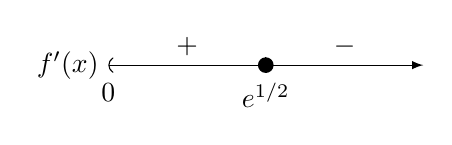
\begin{tikzpicture}
          \draw[(->] (-2,0) -- (2, 0);
          \node[left] at (-2,0) {$f'(x)$};
          \draw[shift={(0,0)},color=black] (0pt,3pt) -- (0pt,-3pt) node[below] {$e^{1/2}$};
          \node[below,yshift=-3pt] at (-2,0) {$0$};
          \node[circle, fill=black, inner sep=2pt] at (0,0) {};
          \node[above] at (-1,0) {$+$};
          \node[above] at (1,0) {$-$};
        \end{tikzpicture}
      \end{center}
      Based on our sign chart, $f(x)$ increases from $x=0$ to $x=e^{1/2}$
      and decreases afterwards, so there is a local maximum at
      $x=e^{1/2}$.

    \end{solution}

  \item
    \begin{problem}[\stretch{0.6}]
      Sketch a graph of $f$. (You need not depict the concavity accurately.) 
    \end{problem}

    \begin{solution}
      We know that the domain of $f$ is $(0, \infty)$. The graph has a vertical asymptote at $x=0$ and
      $\lim\limits_{x\to 0^+} f(x) = -\infty$. $f$ increases
      from $x=0$ to $x=e^{1/2}$ and decreases afterwards. There
      is a horizontal asymptote at $y=0$. So the graph looks
      like this.

      \begin{center}
        \begin{tikzpicture}
          \begin{axis}[restrict y to domain=-4:5,xtick={e^0.5},
          ytick=\empty, xticklabels={$e^{1/2}$}]
            \addplot[domain=0:6] {ln(x)/x^2};
          \end{axis}
        \end{tikzpicture}
      \end{center}
    \end{solution}

  \end{enumerate}

\end{enumerate}
\end{document}
